\documentclass[12pt,oneside]{memoir}

\usepackage[biblatex]{matfmaster}
\usepackage{listings}

\bib{master}

\autor{Милош Самарџија}
\naslov{Развој микросервисне апликације за Android коришћењем окружења Lumen}
\godina{2020}

\mentor{др Милена \textsc{Вујошевић Јаничић}, доцент\\ Универзитет у Београду, Математички факултет}
\komisijaA{др Филип \textsc{Марић}, ванредни професор\\ Универзитет у Београду, Математички факултет}
\komisijaB{др Александар \textsc{Картељ}, доцент\\ Универзитет у Београду, Математички факултет}

% \datumodbrane{ }

% \apstr{ }

\kljucnereci{микросервиси, рачунарство, развојни оквир, андроид, трчање}

\begin{document}

\frontmatter
\naslovna
\komisija
% \posveta{Мојој породици}
% \apstrakt
\tableofcontents*

\mainmatter

\chapter{Увод}
Микросервисна архитектура представљa један од популарнијих приступа развоју скалабилних дистрибуираних система. Главна филозофија на којој је овај приступ заснован је доменски оријентисано моделовање (енг. domain-driven design). Доменски оријентисано моделовање подстиче разбијање комплексних домена на што једноставније и независније поддомене, као и активно учешће доменских експерата (енг. domain experts) у развоју система.

Главна тематика којом се овај рад бави су основне идеје водиље доменски оријентисаног моделовања, на који начин их микросервисна архитектура инкорпорира, као и дизајн REST (енг. representational state transfer) интерфејса за програмирање апликација (енг. RESTful API) који представљa једну од техника за интеграцију поддомена система. У те сврхе је осмишљенa и развијена апликација чији је циљ да илуструје примену микросервисне архитектуре у пракси, као и комуникацију са екстерним сервисима.

Апликација је названа MyRunningBuddy, а њена примарна намена је проналажење партнера за трчање на основу различитих параметара. Сам алгоритам за упаривање тркача уједно представљa и најважнији поддомен (енг. core subdomain) целог система који имплементира пословну логику и на који је потребно обратити највише пажњe током дизајна и имплементације. Део апликације је написан у програмском језику PHP коришћењем Lumen развојног оквира за развој микросервисних апликација и REST интерфејса за програмирање апликација, где је највећи део бизнис логике садржан. Други део апликације је написан у програмском језику Java, заједно са Android комплетом за развој софтвера (енг. Android SDK) и представља кориснички интерфејс, односно улазну тачку у систем, која није у фокусу овог рада, па ће према томе пропорционално мање времена бити утрошено за њен развој. У пракси, корисничка апликација и њен кориснички интерфејс су нешто на шта би подједнако требало обратити пажњу током развоја производа. За потребе складиштењa података од стране микросервиса користи се MySQL база података.
\chapter{Доменски оријентисано моделовање}\label{domenskiorijentisanomodelovanje}
Доменски оријентисано моделовање је филозофија развоја чији циљ је управљање конструкцијом и одржавањем софтвера писаног за комплексне домене. Циљ се достиже употребом одређених образаца (енг. patterns), принципа и добрих пракси које, уколико се добро разумеју и примене, смањују шансу за прављење неких честих грешака које се јављају током развоја.
\section{Чести проблеми развоја пословних апликација}
Да бисмо разумели сврху постојања ове филозофије, потребно је да разумемо на какве изазове се најчешће наилази током развоја и одржавања софтвера. Један од популарнијих архитектуралних стилова коришћених у пословним апликацијама је тзв. велика лопта од блата (енг. Big Ball of Mud) коју карактерише лош дизајн кода са одсуством било какве организације. Такав софтвер је углавном доста спрегнут, и захтев за променом једне од функционалности може изазвати ланчану реакцију других измена које нису планиране, али су у том случају неопходне. Проблем је то што није лако уочљиво када пројекат скрене са правог пута, и од добре архитектуре дође до велике лопте од блата. Са временом се инкрементално квари, додавањем нових функционалности, и крпљењем постојећих, уз слабу бригу о одржању архитектуре, са изговором да ће некад касније бити издвојено време за рефакторисање. Тако настаје технички дуг (енг. technical debt).

Технички дуг је концепт у развоју софтвера настао као еквивалент новчаног дуга. Суштина концепта је да, занемаривањем дизајна кода, дуг постаје све већи, и све је мање вероватно да ће бити успешно измирен. У преводу, долази се до стадијума када је свака измена спецификације (која даље повлачи измене у коду) болна јер је софтвер постао изузетно спрегнут, и много компоненти зависи од других, иако у природи можда чак и не постоји таква веза између тих ентитета. Немогуће је направити изоловане измене, већ су оне раштркане широм система, и због тога се веома лако могу увести нови багови (енг. bugs) у систем. Јасно је да су измене спецификације у пословном софтверу неизбежне, па нам преостаје да се прилагодимо, или да пројекат полако али сигурно одведемо у пропаст. У тој ситуацији се, у зависности од тренутног стања кода, долази до закључка да је неопходно извршити опширно рефакторисање, или дизајнирање и писање софтвера испочетка. То све доводи до већих трошкова за развој, који су се могли избећи.
\section{Идеја филозофије и основни концепти}
Идеја водиља ове филозофије је разбијање великих и комплексних домена на једноставније поддомене. Ово има двојаки значај:
\begin{enumerate}
\item добијамо поддомене који су мање комплексни, и који имају јаснију одговорност
\item лакше се проналази и изолује најважнији поддомен у који је потребно уложити највећи део времена, јер је то оно што одређени софтвер чини другачијим од осталих решења, и представља разлог због којег је уопште и настао
\end{enumerate}

Такође, филозофија инсистира на томе да се у пројекат активно укључе и доменски експерти чија би примарна улога била упознавање програмера и остатка тима са комплексним доменом како би се избегле недоумице и погрешна решења. Ово функционише тако што се током целог развојног циклуса организују формални и неформални састанци са експертима, где се кроз дискусију и различите активности (енг. knowledge crunching) врши анализа и разбијање домена на више мањих, и моделовање поддомена. Као пропратни ефекат ових састанака настају аналитички модел, и заједнички језик (енг. ubiquitous language) чија је улога избегавање двосмислености у комуникацији између експерата и програмера. Током животног циклуса пројекта разумевање домена постаје боље, а заједно са разумевањем се развијају и расту заједнички језик и модели. Сва комуникација, модели и код су изражени у терминима заједничког језика.

\section{Аналитички модел}
Аналитички модел је колекција артефаката који описују модел система, и намена му је да програмерима и пословним корисницима помогне да боље разумеју домен. Да би овај модел имао смисла, све време мора бити усклађен са имплементационим моделом, тј. измене у имплементацији се морају огледати у изменама у аналитичком моделу, и обрнуто. Ова усклађеност постиже се управо изражавањем оба модела у терминима заједничког језика.

Да би се ово остварило, имплементациони модел мора да буде ослобођен било каквих брига које су техничке природе, и да буде фокусиран искључиво на домен. Такође, битно је да аналитички модел буде једноставан за имплементацију, тј. да не буде превише апстрактан, или на превише високом нивоу. Пројекти који постану тешки за одржавање управо пате од недостатка фокуса на домен; технички проблеми бивају помешани са доменском логиком, и дизајн кода се везује за техничке појмове, уместо за домен. То доводи до повећања сложености, и отежаног разумевања пројекта од стране нетехничких лица попут доменских експерата. Комуникација се успорава услед велике количине времена утрошеног на објашњавање техничких концепата нетехничким лицима, врло лако долази до неразумевања и јављају се двосмислености, а потом настају и погрешна софтверска решења.

\section{Врсте поддомена}
Разбијањем комплексног домена открива се више мањих и једноставнијих поддомена са мањим бројем одговорности. Сваки од поддомена се може сврстати у неку од категорија: главни, генерички (енг. generic) и потпорни (енг. supporting) поддомени. Уз сваки добијени поддомен се придружује његов одговарајући модел. Пример разбијања једног комплексног домена на више мањих може се видети на слици \ref{fig:razbijanjedomena}

\begin{figure}[!ht]
  \centering
  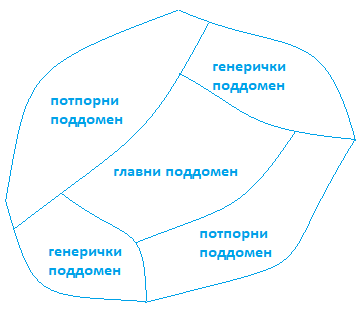
\includegraphics[scale=0.8]{slike/razbijanje-domena.png}
  \caption{Пример поделе комплексног домена на једноставније поддомене}
  \label{fig:razbijanjedomena}
\end{figure}

Под генеричким поддоменом се подразумевају неке од најраспрострањенијих функционалности које и већина других система такође има. Један пример генеричког поддомена може бити подсистем за слање и примање порука. Ово наравно не мора увек бити тачно. Генерички поддомен једног система може бити главни поддомен унутар другог система. У нашем примеру са подсистемом за поруке, у већини система ће вероватно бити сврстан као генерички, али ће представљати главни поддомен у системима чији је највећи адут управо размена порука.

У потпорни поддомен спадају све остале ствари које представљају подршку за функционисање главног домена. Заједничка ствар за потпорне и генеричке домене је то што су у односу на главни поддомен мање битни, али су неопходни јер без њих систем не може бити комплетан.

Главни поддомен садржи највећи и најбитнији део пословне логике, и у зависности од његовог модела и одговарајуће имплементације зависи да ли ће софтвер бити популаран и добро прихваћен, или ће се придружити великом броју других осредњих софтверских решења. Спецификација главног поддомена ће бити најподложнија изменама, и дизајнирању његовог модела треба приступити пажљиво, како би био довољно флексибилан да подржи све накнадне измене.

Са друге стране имамо потпорне и генеричке поддомене чији дизајн може бити слободнији, па се чак могу користити и неке готове софтверске библиотеке (енг. third party libraries). С обзиром да њихов модел не мора бити превише флексибилан, и највероватније ће трпети најмање измена, преживели бисмо и да се неки од њих временом претвори у велику лопту од блата. Кључно је то што је тај лош дизајн изолован од остатка система, и онемогућено му је даље ширење. Уместо претераног фокусирања на потпорне и генеричке поддомене, може се уложити додатни труд у развој главног поддомена. Програмери са мање искуства могу бити задужени за потпорне и генеричке поддомене, а они искуснији могу да се преусмере на главни поддомен.

\section{Доменски модел}
Доменски модел је централни појам доменски оријентисаног моделовања. На почетку се формира у виду аналитичког модела кроз заједничку сарадњу развојног тима и доменских експерата. Не осликава домен у потпуности онако како изгледа у реалности, већ представља поглед на домен из једног угла, односно његову апстракцију, која је довољно добра за наше случајеве употребе. Слика \ref{fig:domenmodelprojekcija} приказује разлику између реалности и самог модела. Модел је описан заједничким језиком којим тим говори, као и дијаграмима које је тим креирао. Садржи само оно што је неопходно у контексту апликације која се креира, и мора да се развија паралелно са пословањем како би био користан и валидан. Модел је користан онолико колико је у стању да представи комплексну логику која решава пословне проблеме, а не колико добро осликава реалност.

Креирање доменског модела није једноставан посао, и представља итеративан процес. Велика је вероватноћа да први добијени модел неће бити задовољавајући, и то не треба да буде обесхрабрујуће. Тим би, заједно са доменским експертима, требало да настави са активностима, у циљу проналажења бољих модела. Не треба се задржати на само једном добром, већ треба пронаћи више задовољавајућих модела. Анализом доменских случајева употребе може се оценити корисност креираног модела, и потврдити да сви чланови тима разумеју домен.

Систем који се конструише се састоји од више целина, где су неке битније од других, па ће постојати и више модела различите сложености који ће се користити у различитим ограниченим контекстима (енг. bounded contexts). С обзиром на захтевност овог процеса, комплексни и богати модели се креирају само за битне поддомене система. 

\begin{figure}[!ht]
  \centering
  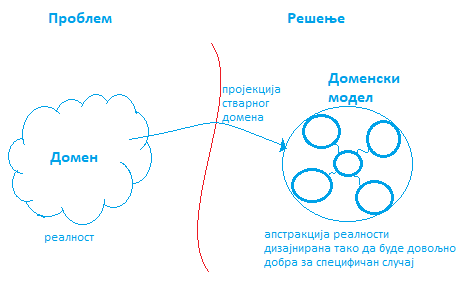
\includegraphics[scale=0.8]{slike/domen-model-projekcija.png}
  \caption{Пројекција реалног домена на једну његову апстракцију}
  \label{fig:domenmodelprojekcija}
\end{figure}
\subsection{Имплементациони обрасци за доменски модел}
Уколико посматрамо слојевите архитектуре софтвера, слој домена би представљао срж апликације. Он изолује сложеност доменског модела од сложености разних техничких делова софтвера. Његова улога је да осигура да се техничке ствари попут логике за управљање трансакцијама, складиштења података и приказивања не умешају у комплексност пословне логике. Мешањем инфраструктурне и пословне логике добили бисмо код који је тежи за разумевање, јер има више од једног задужења, и не можемо се фокусирати на само једну ствар. Слој домена обично представља само мали део целокупне апликације, што се може видети на слици \ref{fig:slojevitaarhitektura}.

\begin{figure}[!ht]
  \centering
  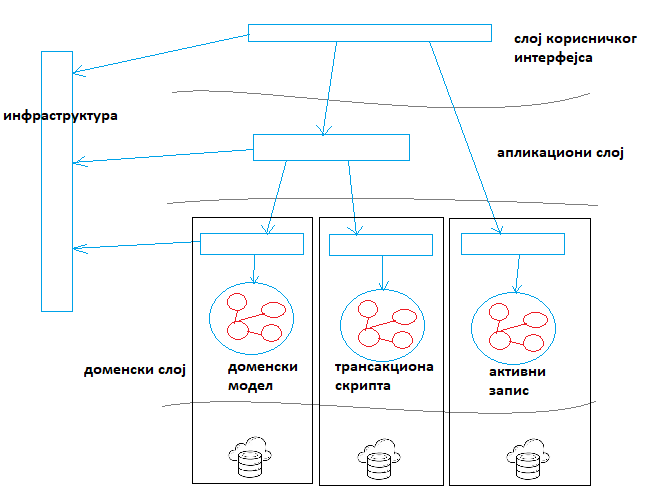
\includegraphics[scale=0.8]{slike/slojevita-arhitektura.png}
  \caption{Слој домена као део сложеније архитектуре}
  \label{fig:slojevitaarhitektura}
\end{figure}

Конструкција доменских модела је проблем који нема јединствено решење, али у пракси постоје одређена решења, односно имплементациони обрасци, који су општеприхваћени и углавном су се добро показали. Неки од њих више одговарају сложенијим поддоменима, док се други могу искористити код једноставнијих, за прављење простијих и сиромашнијих модела. Популарнији обрасци који се користе су доменски модел (енг. domain model), трансакциона скрипта (енг. transaction script) и активни запис (енг. active record).

\subsubsection{Образац "доменски модел"}
Овај образац се најбоље уклапа у комплексне домене са богатом пословном логиком, и подразумева креирање објектно-оријентисаног модела који садржи податке, пословне процесе и правила, и богату доменску логику. Премиса обрасца је да не постоји база података, и да током еволуирања модела проблем складиштења података буде занемарен. Објекти у добијеном моделу су у потпуности ослобођени од инфраструктурних проблема, што нам омогућава да дизајн нашег модела буде фокусиран искључиво на домен. На слици \ref{fig:razdvajanjedomenskogsloja} се може видети како је доменски слој раздвојен од техничких ствари попут складиштења података.

\begin{figure}[!ht]
  \centering
  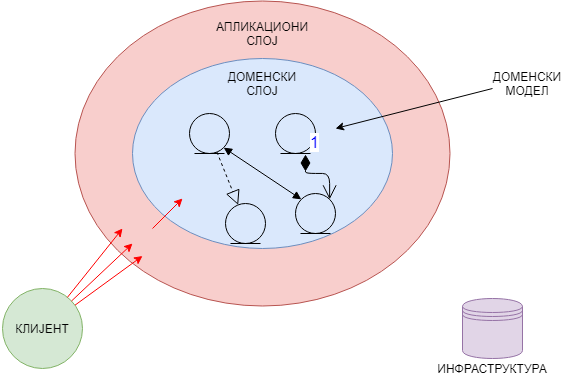
\includegraphics[scale=0.8]{slike/razdvajanje-domenskog-sloja.png}
  \caption{Раздвајање доменског слоја од остатка апликације}
  \label{fig:razdvajanjedomenskogsloja}
\end{figure}

\subsubsection{Образац "трансакциона скрипта"}
Трансакциона скрипта је, за разлику од доменског модела, заснована на процедуралном стилу развоја, лакша је за разумевање и имплементацију. Идеја је да се за сваки пословни случај употребе креира по једна процедура, и да се све те процедуре групишу на једно место. Свака од процедура треба да садржи сву логику потребну да се обави одговарајући случај употребе, укључујући ствари попут пословних правила, логике за складиштење података, итд. Предност овог обрасца су једноставност и могућност да се лако имплементирају нови случајеви употребе додавањем нове процедуре, без бојазни да ли ће бити утицаја на постојећу функционалност. Мане су, очигледно, потенцијално много понављања исте логике на различитим местима и лоша подела одговорности. Овакав образац је најприхватљивији за једноставније поддомене који садрже мало логике.

\subsubsection{Образац "активни запис"}
Активни запис је популарни образац који подразумева да се сваки објекат модела пресликава у одговарајући ред неке табеле. Погодан је у случајевима када модел базе података одговара пословном моделу. Ова структура ће у себи садржати податке и понашање, као и додатне методе за складиштење, додавање нових инстанци и претраживање колекције објеката. С обзиром да свака од структура има методе за креирање, читање, ажурирање и брисање, могуће је коришћење алата и скриптова за аутоматско генерисање доменског модела.

\section{Ограничени контексти и интегритет доменских модела}\label{ogranicenikonteksti}
Већ смо споменули битност разбијања главног домена на неколико мањих. Као резултат тог процеса настају једноставнији поддомени са бољом поделом одговорности, и њихови одговарајући модели. У најбољем случају, пресликавање из поддомена у модел би требало да бијективно; међутим, у пракси се може десити да се неки модели протежу кроз више поддомена, или да један поддомен има више модела. Како би се остварила функционалност система, неопходно је да постоји нека интеракција између добијених модела. Кључно је да модели буду што независнији, и да ова интеракција буде добро дефинисана. У супротном, лако долази до преплитања концепата и логике из различитих поддомена. Да би се заштитио интегритет модела, дефинишу се јасне границе између различитих модела, а то се постиже везивањем модела за одређени контекст, тзв. ограничени контекст.

За разлику од поддомена, који је апстрактан појам, ограничени контексти представљају конкретну техничку имплементацију која ће форсирати одржање граница између модела апликације. Имплементирају се тако да поседују читав стек (енг. stack) функционалности једног поддомена, укључујући презентациони слој, доменску логику и инфраструктуру. Избор архитектуралног обрасца, па и самих технологија за имплементацију једног контекста се може разликовати од контекста до контекста. Сама филозофија не ограничава избор архитектуре, али је потребно да она буде у стању да изолује доменску логику, јер ће се презентација, инфраструктура и доменска логика мењати различитим интезитетом, и из различитих разлога.

Контексти се дефинишу на начин који би омогућио поделу послова између различитих тимова, и тако да унутар једног контекста нема двосмислених појмова који би увели забуну. Природно је да за један ограничени контекст буде задужен само један тим, унутар којег би се развијао заједнички језик. С обзиром да су ограничени контексти доста независни, и комуникацију са другим контекстима обављају преко јасно дефинисаних интерфејса, један тим би јако мало зависио од других тимова, и њихови рокови дистрибуције нових верзија софтвера не би зависили од другог тима и њихових проблема. Ово важи све док се не наруши компатибилност променом интерфејса преко којих се комуникација обавља.

Везе између различитих модела и тимова дефинишу на који начин ће се та комуникација одвијати. У наставку ће бити наведени неки од образаца веза међу контекстима.

\subsection{Антикорупциони слој}
Уколико се комуникација одвија између два ограничена контекста која се одржавају од стране два различита тима, велика је шанса да ће њихови модели бити међусобно некомпатибилни, и да појмови из њихових одговарајућих заједничких језика неће бити изражени на исти начин. Уколико се комуникацији приступи директно, један модел би морао да наруши своју структуру зарад компатибилности са другим моделом, али то се коси са филозофијом да модели треба да буду максимално независни. Најприхватљивије решење је креирање једног слоја индирекције, односно адаптера, који би требало да транслира интерфејс једног модела у интерфејс другог модела. Овај слој се назива антикорупциони слој (енг. anticoruption layer), и омогућава комуникацију између два некомпатибилна интерфејса, без потребе да се један модел прилагођава другом. Примена овог приступа није ограничена само на комуникацију са контекстима других тимова, већ и на комуникацију са екстерним контекстима на чији интерфејс не можемо да утичемо. На овај начин спречавамо да се лош дизајн других компоненти прелије на наш модел.

\subsection{Дељено језгро}
Понекад се може десити да два контекста имају доста заједничких концепата и логике, и покушаји да се они раздвоје могу бити контрапродуктивни, и увести непотребну сложеност. Уместо раздвајања, пракса је да такви контексти деле поједине делове, односно да имају дељени модел преко којег ће се одвијати комуникација. Овај дељени модел се зове дељено језгро (енг. shared kernel). Мана овог приступа је дељени код који уводи зависност, а који је настао као компромис зарад олакшане интеграције. Ово уводи ризик да један контекст може да утиче на интегритет другог, и због тога је потребно обратити додатну пажњу.

\subsection{Узводна/низводна веза}
Веза између два контекста такође може бити дефинисана на основу смера тока података, где ће један контекст бити узводно, а други низводно. У том случају узводни контекст има велики утицај на низводни. Дистрибуције нове верзије узводно ће највероватније имати утицаја на низводне контексте, посебно уколико дође до промене интерфејса.

\section{Слојевита архитектура}
У претходној секцији је речено да архитектура мора да подржи раздвајање доменске логике од остатка апликације, односно раздвајање одговорности. Да би се ово постигло, могу се креирати различити слојеви апликације, где би сваки слој био задужен за неку од одговорности. На слици \ref{fig:inverzijazavisnosti} се може видети слојевита архитектура са доменским слојем у самом језгру. Доменски слој је у потпуности ослобођен било каквих зависности, и фокусиран је искључиво на доменску логику. Апликациони слој који окружује доменску логику има улогу да имплементира пословне случајеве употребе, и то тако што ће оркестрирати доменским моделима и делегирати захтеве доменском слоју. Једина зависност коју апликациони слој треба да има је зависност од доменског слоја.
\begin{figure}[!ht]
  \centering
  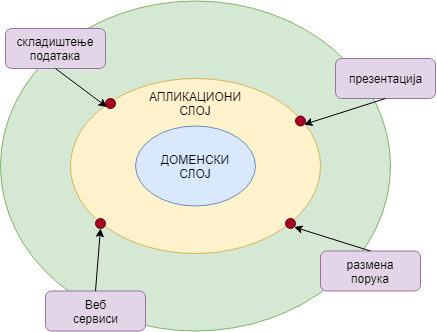
\includegraphics[scale=0.8]{slike/inverzija-zavisnosti.png}
  \caption{Слојевита архитектура апликације са инверзијом зависности}
  \label{fig:inverzijazavisnosti}
\end{figure}

Јасно је да ће ова два слоја имати потребу за складиштењем података, и за разним другим инфраструктурним услугама. Да би се ово остварило без увођења додатне зависности, примењује се принцип познатији као инверзија зависности (енг. dependency inversion). Инверзија зависности у овом случају подразумева да, уместо да се апликациони слој прилагођава специфичностима сваке инфраструктурне услуге, свака од услуга имплементира унапред дефинисан интерфејс од стране апликационог слоја. Пропратни ефекат независности апликационог и доменског слоја од остатка апликације је њихово олакшано тестирање, тј. тестирање пословне логике у изолацији, без инфраструктурних зависности.

\section{Интеграција ограничених контекста}\label{integracijaogranicenihkonteksta}
У секцији \ref{ogranicenikonteksti} смо видели неке од веза између контекста који међусобно интерагују. Сваки од ограничених контекста може представљати засебан процес који може бити извршаван на различитим физичким машинама. Добра ствар овог приступа где су различити контексти засебни процеси је то што је апликација отпорнија на отказивање одређених компоненти система, па чак и на саме физичке кварове. Додатно, софтвер је скалабилнији. У случају повећаног броја корисника, а самим тим и количине операција који се обрађује од стране апликације, софтвер мора бити у стању да се скалира како би успешно опслужио све кориснике.

Једно од решења је вертикално скалирање, које подразумева повећање хардверских ресурса на једној машини, попут радне меморије, складиштног простора, и броја процесора. Јасно је да овај приступ има ограничење, и да повећање ресурса на тај начин не може бити дугорочно решење. Боље решење је да апликација буде способна да се скалира хоризонтално, односно, да са порастом оптерећења система додајемо нове физичке машине у нашу инфраструктуру, и да покрећемо додатне инстанце софтвера. Међутим, по правилу су овакви системи доста сложенији. С обзиром да апликација није монолитна, већ је дистрибуирана у различитим процесима, који се могу налазити на различитим физичким локацијама, и самим тим је комуникација дистрибуираних делова апликације сложенија. Потребно је дефинисати на који начин ће те компоненте бити интегрисане, како ће се синхронизовати, а јавља се и питање конзистентности. Сви наведени проблеми представљају нешто са чиме се сваки дистрибуирани систем суочава, и од система до система се могу разликовати реализована решења, а у зависности од случајева употребе, природе самог домена, и очекивања корисника.

Нека од конкретних техничких решења која могу бити употребљена за комуникацију унутар оваквог система су интеграција коришћењем базе података, интеграција помоћу датотека, позив удаљене процедуре (енг. remote procedure call), интеграција коришћењем система за размену порука (енг. messaging) и REST интерфејси за програмирање апликација.

\subsection{Интеграција коришћењем базе података}
Интеграција коришћењем базе података представља најједноставнији вид интеграције ограничених контекста који подразумева да једна компонента упише нешто у базу података, а да онда друга компонента то прочита. Ово читање би могло да буде имплементирано тако да компонента која чита врши читање на сваких неколико секунди или минута. Иако није захтевно за имплементацију, ово решење поседује и неке мане због којих је прихватљиво употребити га само у некритичним деловима система или у првобитним итерацијама. Неки од проблема који се јављају код оваквог типа интеграције је то што су компоненте спрегнуте са базом података. Уколико једна компонента има захтев за променом схеме базе података, друга компонента би морала да се прилагоди тој новој схеми. Такође, код база података као потенцијални проблем се јавља и закључавање које се поприлично може одразити на перформансе уколико један део апликације нпр. интезивно уписује у базу, а други део врши ажурирање. Поред тога, код овакве интеграције база је критична тачка пуцања. Уколико база није доступна, комуникација између компоненти ће бити онемогућена. 

\subsection{Интеграција помоћу датотека}
Овај тип интеграције је доста сличан интеграцији коришћењем базе података. Уместо да део апликације податке уписује у базу података, може их уписати у неку датотеку, из које касније друга компонента може да чита. Овакво решење је некад пожељније у односу на претходно, посебно уколико би апликација базу података користила искључиво за интеграцију. Уместо конфигурисања базе података, у том случају је једноставније податке размењивати преко неке датотеке. Овакав приступ нема проблема са закључавањем, али ипак не нуди решење за скалирање, што значи да би приликом имплементације таквог решења требало осмислити неки механизам за скалирање, редудантност, као и формат самих датотека.Њ

\subsection{Позив удаљене процедуре}
Позив удаљене процедуре је популаран и често коришћен начин интеграције. У основи, комуникација између две компоненте се обавља посредством рачунарске мреже, коришћењем неког протокола, најчешће HTTP. Идеја је да се од програмера прикрије чињеница да су компоненте физички удаљене, и да се комуникација одвија преко мреже. Летимичним погледом на код се не може закључити да се ради о мрежној апликацији, јер је сама сложеност мрежне комуникације скривена, а позиви метода, као и њихова имена ни на који начин не откривају да се не ради о монолитној апликацији. У позадини, ово се изводи тако што се за методе које представљају удаљене процедуре генерише клијентски и серверски код. Он између осталог садржи логику за серијализацију и десеријализацију параметара и позиве мрежних функција. Позив метода у клијентској апликацији проузрокује да се порука са информацијом о методу који се позива и листом параметара серијализује у низ бајтова, и онда се шаље кроз мрежу. На серверској страни се порука прима, десеријализују се назив метода и његови параметри, и извршава се одговарајући удаљени код. Транспарентност овог начина интеграције уједно може бити и његова мана. Врло је лако заборавити да се ради о мрежним позивима, па њихово неоптимално и пречесто позивање може довести до проблема са перформансама. Такође, позиви удаљених процедура су проблематични уколико постоји захтев да се неки код извршава асинхроно. У том случају, боље решење представља коришћење система за размену порука. 

\subsection{Интеграција коришћењем система за размену порука}
Интеграција коришћењем система за размену порука се користи у апликацијама чије компоненте би требало да комуницирају асинхроно. Систем за размену порука је најчешће имплементиран као дистрибуирани ред који има могућност да се скалира, реплицира податке и шаље их кроз мрежу, и може се посматрати као засебна компонента. У односу на позив удаљених процедура, овај метод интеграције је отпорнији на отказивање компоненти, јер савремени системи за размену порука имају могућност чувања порука које нису послате, у случајевима када постоје мрежни проблеми, или уколико компонента која прима поруке привремено није активна, као и поновно слање тих порука када је систем поново стабилан. Када нека компонента жели да шаље поруке, шаље их у виду догађаја (енг. events), заједно са додатним подацима неопходним за обрађивање тог типа догађаја. Компоненте заинтересоване за одређени тип догађаја се могу претплатити (енг. subscribe) на исти. На овај начин компонента која врши слање уопште не мора да зна ко све прима поруку, већ ће компоненте које желе да обрађују одређени тип догађаја претплатом изразити интересовање. Мана овог приступа је то што се подразумева употреба асинхроне парадигме, која је скоро увек захтевнија за имплементацију и разумевање јер се доста разликује од конвенционалног синхроног програмирања. Такође, захтева посматрање проблема из другачијег угла, као и сасвим другачији дизајн компоненти.

\subsection{REST интерфејси за програмирање апликација}
REST интерфејси су интерфејси за програмирање апликација који су имплементирани у складу са REST архитектуралним стилом и омогућавају комуникацију са удаљеним сервисима. Дизајнирани су тако да могу да искоришћавају постојеће протоколе. Најчешће се користи HTTP, али у теорији се може користити било који протокол. Због тога није неоподна инсталација додатних библиотека и додатног софтвера. Неки од критеријума које интерфејс мора да задовољи да би био у складу са REST архитектуралним стилом су:
\begin{enumerate}
\item клијентско-серверска архитектура која се састоји од клијената, сервера и ресурса
\item комуникација између клијената и сервера је без стања, односно, сервери не чувају информације о клијентима између различитих захтева (непостојање сесије)
\item сваки ресурс мора бити јединствено идентификован, и њихова интерна репрезентација треба бити раздвојена од репрезентације која се шаље клијентима
\item репрезентација ресурса коју добија клијент мора да садржи довољно информација које ће омогућити манипулацију самим ресурсом, као и довољно информација о томе како би клијент требало да процесира поруку
\end{enumerate}
Формат захтева и одговора није дефинисан самим архитектуралним стилом, и може се користити формат по избору. С обзиром да ће креирана апликација користити управо овај тип интеграције, у наредним секцијама ће бити више речи о самом дизајну REST интерфејса. 

\chapter{Микросервисна архитектура}
Микросервиси представљају архитектурални стил којег одликују мали, независни сервиси који раде заједно како би обавили неки посао. Због сличности, неретко долази до мешања термина микросервиса и доменски оријентисаног моделовања. Та сличност потиче од чињенице да доменски оријентисано моделовање представља само филозофију развоја, односно скуп препорука, образаца и циљева, док су микросервиси једно конкретно решење како се та филозофија може применити у стварности.

Разбијањем апликације на мање, добро дефинисане сервисе, микросервиси деле проблем који тај софтвер решава на једноставније потпроблеме. Тако се придржавају принципа разбијања домена на мање поддомене који је описан у поглављу \ref{domenskiorijentisanomodelovanje}. Сва комуникација се одвија преко мрежних позива, који су скупе операције, и форсира се што већа раздвојеност међу сервисима; на тај начин се смањује опасност од велике спрегнутости. Независност и мала спрегнутост омогућавају да се мењање једног сервиса и дистрибуција нових верзија обављају независно у односу на остале сервисе.

Сваки сервис дефинише интерфејс за програмирање апликација преко којег остали сервиси могу да комуницирају са њим. Раздвојеност сервиса програмерима даје слободу да користе различите програмске језике у различитим сервисима, па технологија која се користи за интерфејс треба да буде језички неутрална (енг. language-agnostic), односно да не ограничава избор програмског језика. Поред коришћења различитих програмских језика, различите компоненте такође могу да користе и различите механизме за трајно складиштење података. На пример, један сервис може да буде имплементиран у C++ програмском језику и да користи релациону базу података, а неки други може да буде имплементиран у Пајтону (eng. Python) и да за складиштење користи обичну датотеку. Предност овога је то што се избор технологије може вршити у зависности од природе поддомена и потребних перформанси, преференција особе или тима задуженог за одређени сервис, и слично. Додатно, мање битни сервиси могу да експериментишу са новим технологијама, без страха да ће се евентуални проблеми прелити на остатак система. И наравно, пошто су сервиси мали, врло је лако поново их имплементирати у неком другом програмском језику уколико нова технологија не испуни очекивања.   

\section{Предности и мане микросервиса}
С озбиром да се ради о независним сервисима, јасно је да микросервиси потпадају у категорију дистрибуираних система. Самим тим наслеђују њихове предности и мане. Неке од предности дистрибуираних система су редудантност и отпорност на отказивање, боље скалирање, олакшано распоређивање (енг. deployment) и бржи одзив. Ипак, иако због свега овога звуче као добро решење за сваки проблем, микросервиси имају и отежавајуће околности довољно велике да није исплативо користити их уколико природа самог проблема који се решава не захтева то. Пре свега, ту се мисли на безбедност, проблеме са конзистентношћу и теже детектовање проблема.

\subsection{Скалирање}
У секцији \ref{integracijaogranicenihkonteksta} смо видели да постоје два типа скалирања. Видели смо и разлоге зашто се преферира хоризонтално скалирање у односу на вертикално. Код поддомена који су по природи погодни за паралелизацију постоји могућност покретања више инстанци истог сервиса како би се оптерећење са једне инстанце једнако распоредило на више њих. Број инстанци једног сервиса је динамички, односно, у току већег налета захтева ка систему, покрећу се додатне инстанце како би се избегло оптерећење и успорена обрада података. Када се број захтева врати у нормалу, додатне инстанце се искључују. Ово додавање и избацивање нових инстанци се може обављати ручно, али може бити и аутоматизовано, тако што ће се број инстанци регулисати на основу статистике, нпр. на основу броја активних корисника, захтева у секунди, одзива и слично. Једна од најбитнијих ствари које корисници система захтевају је то да добијају одговоре на њихове захтеве у што краћем року.

\subsection{Редудантност и отпорност на отказивање}
Кренимо прво од монолитних апликација, и упоредимо њихову отпорност на отказивање у односу на микросервисе. Уколико један модул монолитне апликације услед неког проблема откаже, нпр. референцирањем показивача на невалидну меморијску локацију, цела апликација насилно завршава са извршавањем. Такође, ако дође до отказивања физичке машине, једна једина инстанца апликације са којом је корисник имао интеракцију престаје да постоји. Укратко, отпорност на овакве врсте отказа не постоји.

За разлику од монолитне апликације, отказивање једног сервиса у микросервисној архитектури не утиче на доступност осталих сервиса, било да се ради о отказивању сервиса услед неке грешке, или о отказивању физичке машине (ово важи ако се сви сервиси не налазе на истој машини). Један од начина како се микросервисна архитектура бори са оваквим проблемима је да након отказивања систем може да пређе у другачији режим рада, са редукованим функционалностима док се проблематични сервис поново не подигне.

Други начин је постојање резервних (енг. backup) инстанци које би могле да замене инстанцу која више није активна. Резервне инстанце могу бити активне и у стању приправности све време у току рада примарне инстанце, a могу бити и искључене, и покренуте по потреби; то је тзв. хладна резерва (енг. cold backup). Хладна резерва се користи у ситуацијама кад је подизање сервиса брзо, или је период неактивности док се сервис подиже прихватљиво. Предност хладних резерви је у томе што примарни и резервни сервиси нису активни истовремено, па самим тим утрошак ресурса није дупло већи.

Било да се користе активне или хладне резерве, потребно је да постоји механизам који би могао да утврђује да ли је примарна инстанца активна или није, и да ли је у стању да обрађује захтеве, и да покреће резервне инстанце уколико је потребно. Овај механизам мора радити поуздано, како би се избегла ситуација где и примарна и резервна инстанца активно прихватају и обрађују захтеве; таква ситуација је опаснија од тоталне неактивности, јер може нарушити стање целог система. Једно од софтверских решења које се користи у ове сврхе је Apache ZooKeeper.

\subsection{Распоређивање}
Распоређивање софтвера представља све активности које је неопходно обавити како би се апликација оспособила за употребу. То укључује дистрибуцију нове верзије, инсталацију и конфигурисање, деинсталацију и ажурирања. Ситне промене у комплексним монолитним апликацијама захтевају да се изврши распоређивање целе апликације. Распоређивање велике апликације представља процедуру која носи огроман ризик, па се у пракси овако ризичне процедуре дешавају што је ређе могуће; пре распоређивања се обично скупи доста измена, које се онда дистрибуирају кроз исту верзију. У међувремену су корисници могли да промене мишљење и да одлуче да ипак не желе неку функционалност, или су одлучили да желе да нешто функционише другачије. Услед нагомиланих измена, теже је селективно поништити само неке од измена, посебно јер можда те измене зависе од неких других.

Код микросервиса је прича једноставнија. Сервис у којем су направљене измене се може распоредити независно од осталих сервиса у систему. Лакше се поништавају направљене измене у случају проблема, а и сам проблем је изолован од остатка система. Такође, нове измене се дистрибуирају много брже.

\subsection{Одзив}
Већ смо рекли да је одзив јако битна карактеристика која може утицати на задовољство корисника. Ово не зависи увек само од оптерећења система, већ и од тога где су корисници географски лоцирани у односу на сам систем. Систем може бити растерећен, али уколико је корисник на другом крају света, спорији одзив услед пропагације података кроз мрежу се не може избећи. Ово се решава тако што се покреће више инстанци истог сервиса, али на различитим локацијама широм света. Балансери захтева на основу локације корисника онда могу да одаберу физички најближи сервис са којим ће корисник комуницирати.

\subsection{Безбедност}
Током развоја софтвера је изузетно битно да се пажња обрати и на безбедност, посебно уколико се ради о софтверу високог значаја. Дистрибуирани системи за комуникацију интезивно користе рачунарске мреже, што ствара додатне слабе тачке које је потребно заштитити. Поред стандардних пропуста који се јављају код једнопроцесних апликација, рачунарске мреже отварају нове могућности за искоришћавање система у сврхе које су изван дефинисаних случајева употребе, међу којима су и оне малициозне. Главна линија одбране би требало да буде добро исконфигурисана мрежа која би спречила евентуалне упаде уљеза, али и поред тога, сва комуникација међу сервисима би требало да се одвија као да ће потенцијални уљези пробити заштитну баријеру мреже. То подразумева да би већина саобраћаја (ако не и сав саобраћај) требало да буде енкриптована, посебно део комуникације који може садржати осетљиве податке, попут лозинки, бројева картица, и слично.

Код дистрибуираних система код којих су перформансе од великог значаја, посебно код система који раде у реалном времену, енкрипција података може представљати проблем. Криптографске функције могу створити додатни утрошак (енг. overhead) драгоцених ресурса, посебно уколико се користе јачи алгоритми за енкрипцију. У том случају, уместо шифровања свих података у систему, могу се шифровати само осетљиви подаци, као и комуникација између клијената и самог система.

\subsection{Конзистентност}
Постојањем више раздвојених сервиса, добијамо бољи одзив и скалирање, и апликација је отпорнија на отказивање, али се јављају проблеми са конзистентношћу. Конзистентност подразумева да захтев за неким подацима ка било којем сервису унутар система увек враћа најсвежије податке. Пропагација података кроз цео систем захтева одређено време, и јасно је да решење овог проблема не може бити савршено, већ мора постојати неки компромис. Ова тема ће бити детаљније обрађена у секцији...

\subsection{Детектовање проблема}
Надгледање софтвера у продукцији и детектовање евентуалних проблема је изузетно важан процес. Информациони системи од великог значаја не трпе дуготрајне периоде неактивности, и све потенцијалне проблеме је потребно детектовати на време, и одреаговати што пре. Код монолитних апликација, овај задатак је релативно праволинијски, и подразумева праћење логова, надгледање живости и здравља саме апликације, и то најчешће може бити аутоматизовано. Код микросервиса је ово мало сложеније, због многобројних сервиса које је потребно пратити. Истовремено је потребно пратити стање свих активних инстанци сервиса у систему, на различитим физичким и виртуелним машинама, и овде је аутоматизација неопходна; свако друго решење је непродуктивно. Ручно праћење логова и проверавање појединачних сервиса би захтевало много времена и велики фокус. Додатно, поред здравља појединачних сервиса, потребно је обратити пажњу и на стање мреже која омогућава комуникацију и сарадњу сервиса. Да би се овај задатак аутоматизовао, мора постојати механизам откривања сервиса (енг. service discovery) који би могао да детектује динамичне промене у инфраструктури, попут додавања нових инстанци и њиховог уклањања.

\section{Распоређивање}
\subsection{Континуална интеграција}

\section{Тестирање}

\section{Надгледање}

\section{Безбедност}

\section{Скалирање}

\chapter{Дизајнирање REST интерфејса}

\chapter{Lumen развојни оквир}

\chapter{Android}

\chapter{Практични део рада}

\chapter{Закључак}

\literatura

% \backmatter

\end{document} 
